\begin{lstlisting}
chapter 6: 12 17 19 20
chapter 7: 2 3
\end{lstlisting}
\begin{exercise}
\begin{figure}[H]
\centering
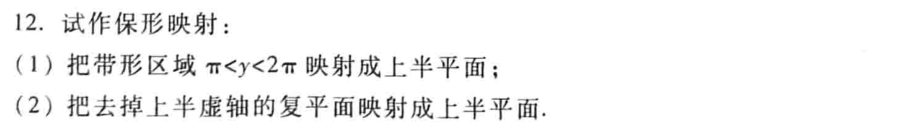
\includegraphics[width=\textwidth]{hw14-2025052917.png}
% \caption{}
\label{}
\end{figure}
\end{exercise}
(1) $w=-e^{ z }$.

(2) $w=(-iz)^{1/2}$.

\begin{exercise}
\begin{figure}[H]
\centering
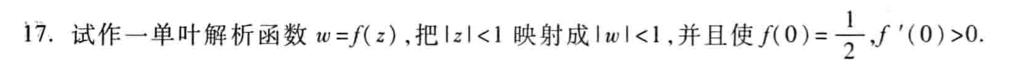
\includegraphics[width=\textwidth]{2-hw14-2025052917.png}
% \caption{}
\label{}
\end{figure}
\end{exercise}
\[
f(z)=\frac{\frac{1}{2}+z}{1+\frac{z}{2}}
\]
Then for any $\lvert z \rvert<1$,
\[
\lvert f(z) \rvert ^2=\frac{\frac{1}{2}+z}{1+\frac{z}{2}}\cdot \frac{\frac{1}{2}+\overline{z}}{1+\frac{\overline{z}}{2}}=\frac{\frac{1}{4}+\lvert z \rvert ^2+\frac{1}{2}(z+\overline{z})}{1+\frac{1}{4}\lvert z \rvert ^2+\frac{1}{2}(z+\overline{z})}=1+\frac{\frac{3}{4}(\overbrace{ \lvert z \rvert ^2-1 }^{ <0 })}{\underbrace{ 1+\frac{1}{4}\lvert z \rvert ^2+\frac{1}{2}(z+\overline{z}) }_{ =\left\lvert  1+\frac{z}{2}  \right\rvert ^2>0 }}<1
\]
Then $\lvert f(z) \rvert<1$. For $\lvert z \rvert=1$, we have $\lvert f(z) \rvert=1$. Observe that
\[
f(0)=\frac{1}{2}\qquad f\left( -\frac{1}{2} \right)=0
\]
Then $g\coloneqq -f(-f(z))$, maps $\mathbb{D}$ into $\mathbb{D}$, and
\[
g(0)=-f(-f(0))=-f\left( -\frac{1}{2} \right)=0\qquad g\left( -\frac{1}{2} \right)=-f\left( -f\left( -\frac{1}{2} \right) \right)=-f(0)=-\frac{1}{2}
\]
By the Schwarz lemma, $g:z\mapsto ze^{ i\theta }$, and $\theta=0$. Thus $g$ is identity map of $\mathbb{D}$, thus $f$ is automorphism of $\mathbb{D}$. Also
\[
f'(z)=\frac{1}{1+\frac{z}{2}}-\frac{\frac{1}{2}\left( \frac{1}{2}+z \right)}{\left( 1+\frac{z}{2} \right)^2}
\]
Then $f'(0)=1-\frac{1}{4}=\frac{3}{4}>0$. We are done!

\begin{exercise}
\begin{figure}[H]
\centering
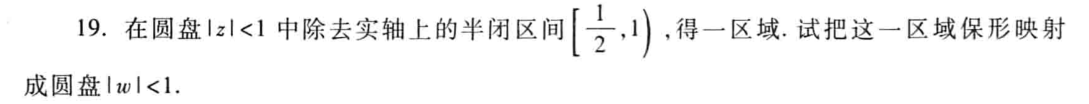
\includegraphics[width=\textwidth]{3-hw14-2025052917.png}
% \caption{}
\label{}
\end{figure}
\end{exercise}
\begin{figure}[H]
\centering
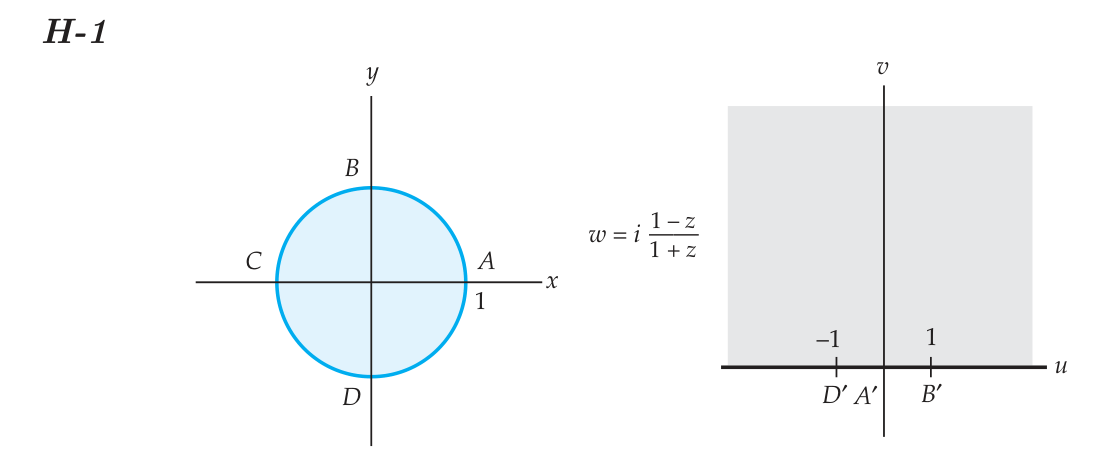
\includegraphics[width=\textwidth]{1-hw14-2025052918.png}
% \caption{}
\label{}
\end{figure}
\begin{figure}[H]
\centering
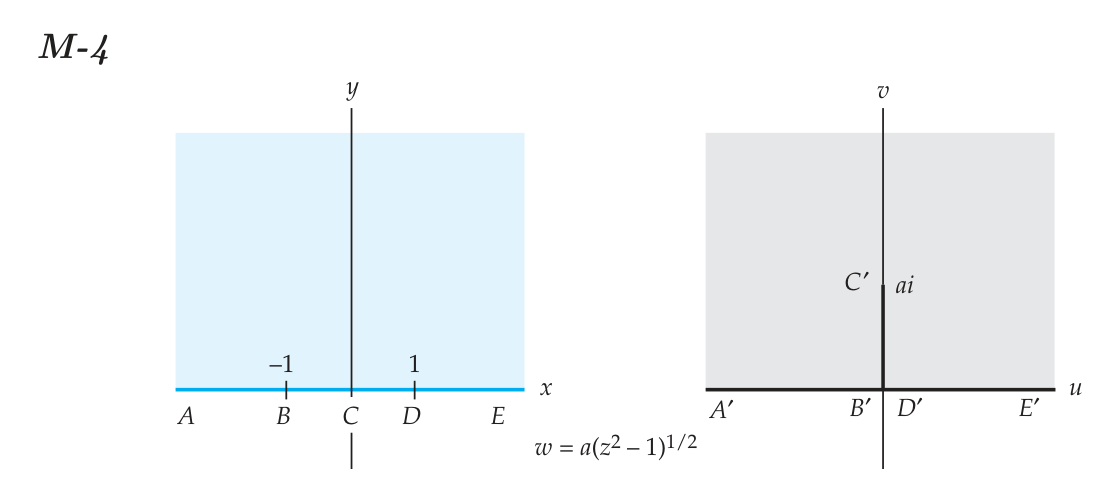
\includegraphics[width=\textwidth]{hw14-2025052918.png}
% \caption{}
\label{}
\end{figure}
\begin{figure}[H]
\centering
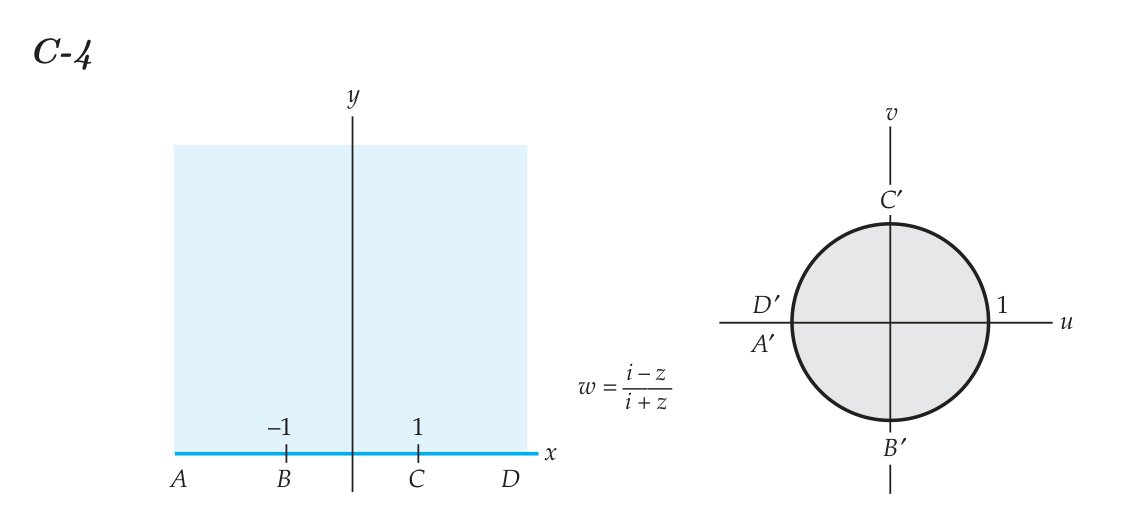
\includegraphics[width=\textwidth]{2-hw14-2025052918.png}
% \caption{}
\label{}
\end{figure}

\begin{figure}[H]
\centering
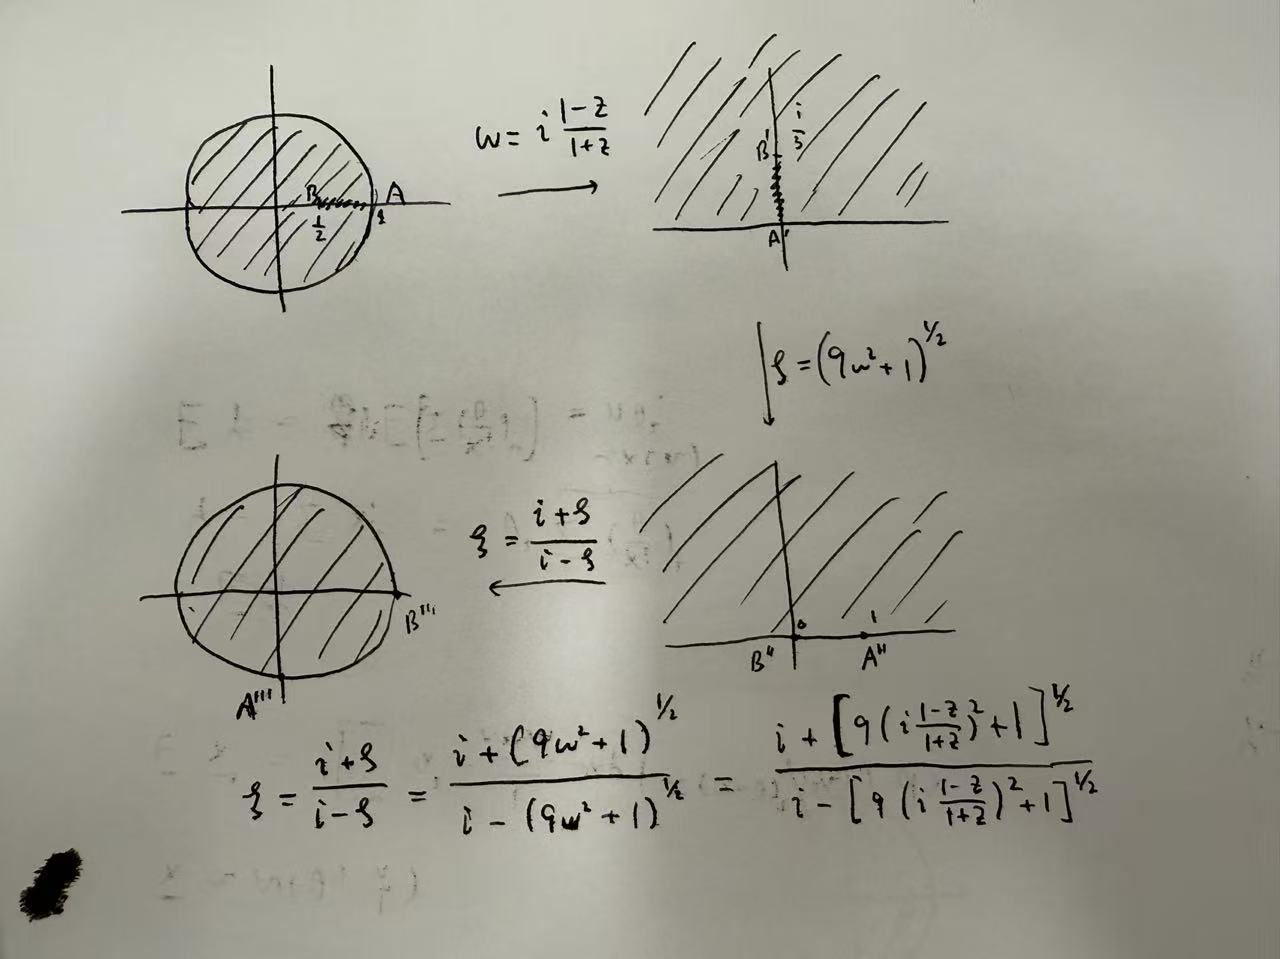
\includegraphics[width=\textwidth]{a393006df0620aef45a9b6a80d90478e.jpg}
% \caption{}
\label{}
\end{figure}
\[
\xi=\frac{i+\left[ 9\left( i\frac{1-z}{1+z} \right)^2+1 \right]^{1/2}}{i-\left[ 9\left( i\frac{1-z}{1+z} \right)^2+1 \right]^{1/2}}
\]
\begin{exercise}
\begin{figure}[H]
\centering
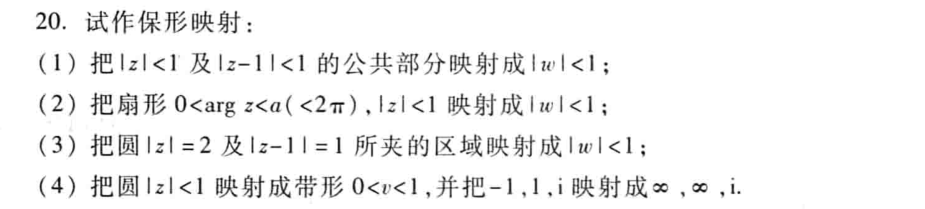
\includegraphics[width=\textwidth]{4-hw14-2025052917.png}
% \caption{}
\label{}
\end{figure}
\end{exercise}
(1)
\begin{figure}[H]
\centering
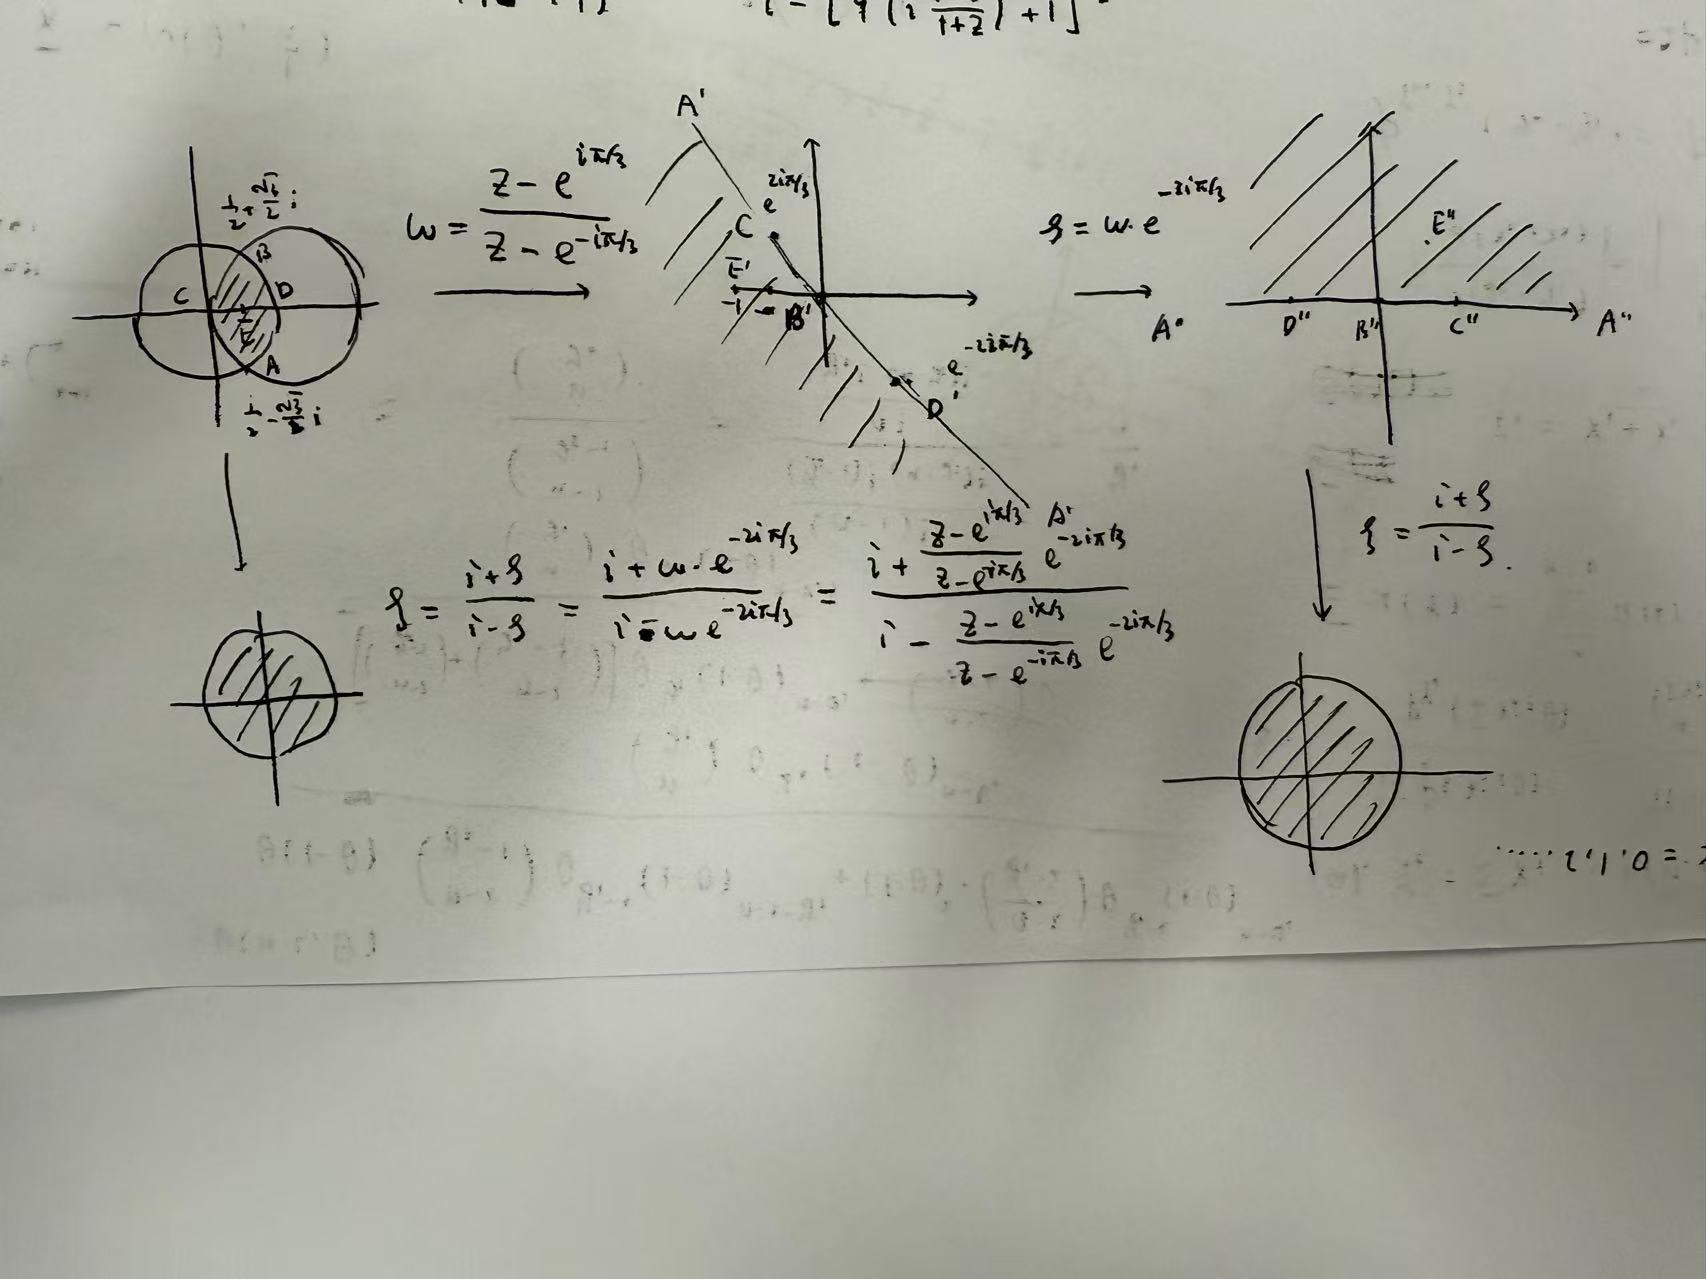
\includegraphics[width=\textwidth]{17d48dfe08a8c60e7a8d5dd893bf3c98.jpg}
% \caption{}
\label{}
\end{figure}
\[
\xi=\frac{i+\frac{z-e^{ i\pi/3  }}{z-e^{ i\pi/3 }}e^{ -2i\pi/3  }}{i-\frac{z-e^{ i\pi/3  }}{z-e^{ i\pi/3 }}e^{ -2i\pi/3  }}
\]
(2)
\begin{figure}[H]
\centering
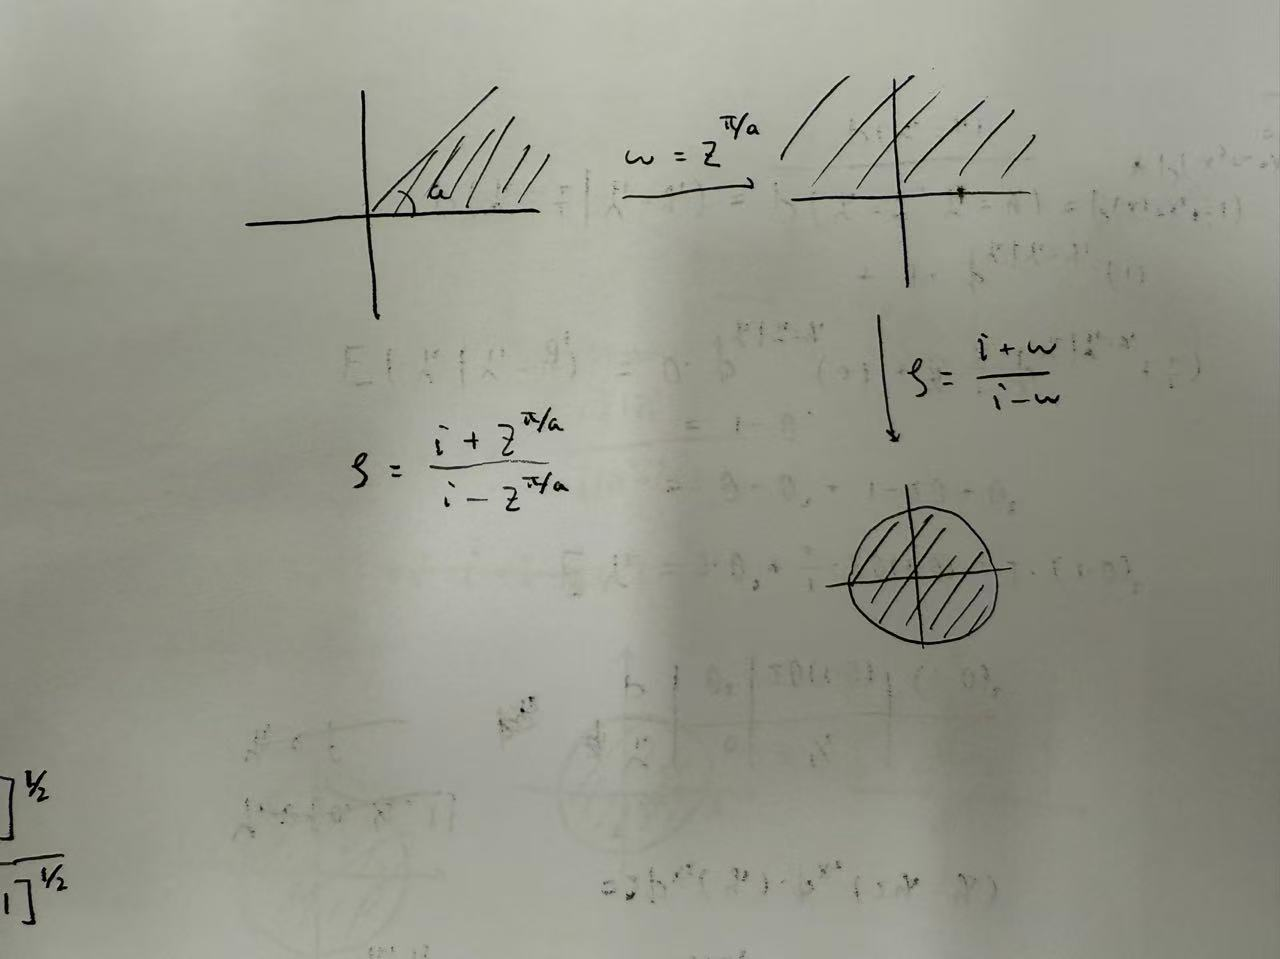
\includegraphics[width=\textwidth]{66bd5be75a90d9827be52563390c9f9c.jpg}
% \caption{}
\label{}
\end{figure}
\[
\zeta=\frac{i+z^{\pi/a }}{i-z^{\pi/a}}
\]
(3)
\begin{figure}[H]
\centering
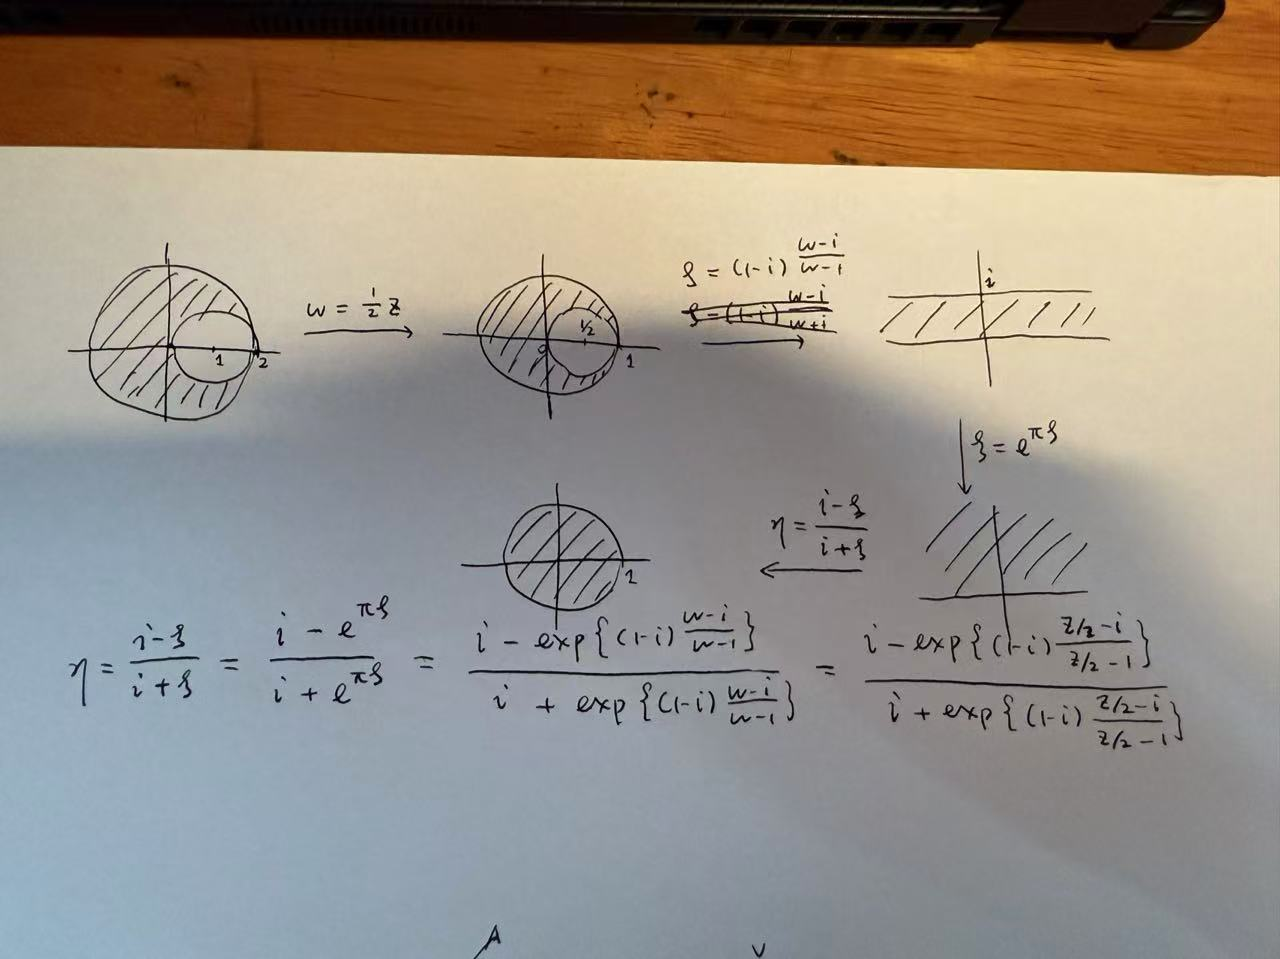
\includegraphics[width=\textwidth]{ba4917f1a31f5671aee9ccca4f690827.jpg}
% \caption{}
\label{}
\end{figure}
\[
\eta=\frac{i-\exp \left\{  (1-i)\frac{\frac{z}{2}-i}{\frac{z}{2}-1}  \right\}}{i+\exp \left\{  (1-i)\frac{\frac{z}{2}-i}{\frac{z}{2}-1}  \right\}}
\]
(4)
\begin{figure}[H]
\centering
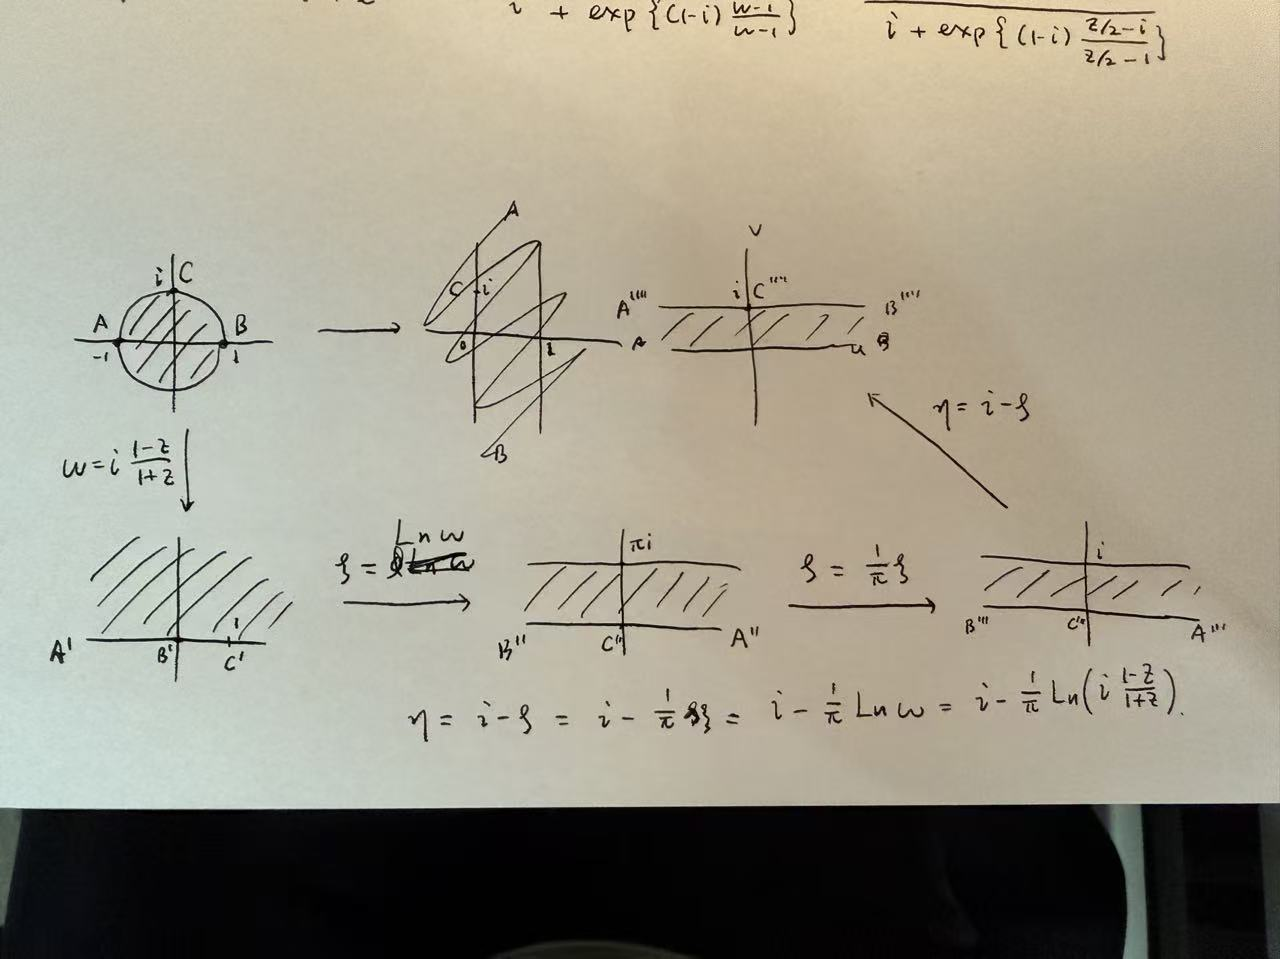
\includegraphics[width=\textwidth]{5e8abe1cfe7bb61cc10f4bf33db4c4cf.jpg}
% \caption{}
\label{}
\end{figure}
\[
\eta=i-\frac{1}{\pi}\mathrm{Ln}\left( i\frac{1-z}{1+z} \right)
\]
\begin{exercise}
\begin{figure}[H]
\centering
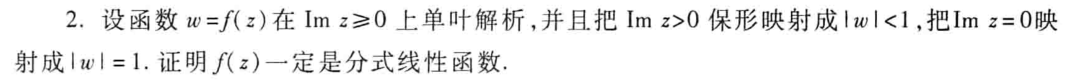
\includegraphics[width=\textwidth]{5-hw14-2025052917.png}
% \caption{}
\label{}
\end{figure}
\end{exercise}
\begin{figure}[H]
\centering
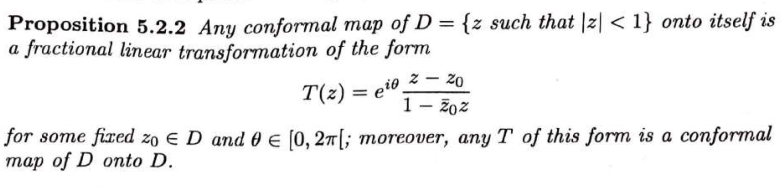
\includegraphics[width=\textwidth]{1-hw14-2025052922.png}
% \caption{}
\label{}
\end{figure}

考虑共形映射
\[
g:\overline{\mathbb{D}}\to \{ \text{Im }z\geq 0 \}\qquad z\mapsto i\frac{1-z}{1+z}
\]
\[
h:\{ \text{Im }z\geq 0 \}\to \overline{\mathbb{D}}\qquad z\mapsto\frac{i-z}{i+z}
\]
他们互为逆映射,由于 $\left.f\right|_{\{ \text{Im }z>0 \}}$ 的值域为 $\mathbb{D}$,$\left.g\right|_{\mathbb{D}}$ 的值域为 $\{ \text{Im }z>0 \}$,于是 $f\circ g$ 是 $\mathbb{D}$ 的自同构,且为共形映射. 从而
\[
f(g(z))=e^{ i\theta }\frac{z-z_0}{1-\overline{z_0}z},\qquad \forall z\in \mathbb{D}
\]
于是
\[
\left.f\right|_{\{ \text{Im }z>0 \}}(z)=e^{ i\theta }\frac{h(z)-z_0}{1-\overline{z_0}h(z)}
\]
是分式线性映射. 由唯一性原理可知,$f$ 是分式线性映射.


单叶解析函数和共形映射是复变函数理论中的两个重要概念,它们之间有密切的联系,但含义不同。

\textbf{单叶解析函数}

一个函数 $f(z)$ 如果在区域 $D$ 内是解析的,并且对于 $D$ 中任意不同的两点 $z_1 \neq z_2$,都有 $f(z_1) \neq f(z_2)$,则称 $f(z)$ 在 $D$ 内是单叶的(或单价的、单射的)。

简单来说,单叶就是指函数在定义域内是一对一的(injective)。这是函数的一个\textbf{整体性质}。

\textbf{共形映射}

一个函数 $f(z)$ 如果在区域 $D$ 内是解析的,并且对于 $D$ 内的每一点 $z_0$,它都保持经过 $z_0$ 的任意两条光滑曲线的夹角大小和定向不变,则称 $f(z)$ 在 $D$ 内是共形的。

解析函数保持角度和定向的充要条件是其在该点的导数不为零。所以,一个解析函数 $f(z)$ 在 $D$ 内是共形的,等价于 $f(z)$ 在 $D$ 内是解析的且对于所有的 $z \in D$,都有 $f'(z) \neq 0$。

共形性是函数的一个\textbf{局部性质}(在每一点 $z_0$ 附近保持角度)。

\textbf{区别与联系}

\begin{enumerate}
	\item \textbf{定义不同:} 单叶强调的是函数的整体一对一性;共形强调的是函数在每一点的局部保角和保向性(对于解析函数,等价于导数不为零)。
	\item \textbf{性质包含:}
	\begin{itemize}
		\item 如果一个解析函数在区域 $D$ 内是\textbf{单叶}的,那么它在该区域内一定是\textbf{共形}的。这是因为,如果 $f(z)$ 是单叶解析的,可以证明其导数在 $D$ 内不可能为零(如果 $f'(z_0)=0$ 且 $z_0$ 是零点,解析函数的零点是孤立的,局部上函数行为类似 $c(z-z_0)^m$ ($m \geq 2$), 这会破坏单叶性)。而解析且导数不为零正是共形的定义。
		\item 然而,如果一个解析函数在区域 $D$ 内是\textbf{共形}的(即解析且 $f'(z) \neq 0$),它\textbf{不一定}是\textbf{单叶}的。例如,函数 $f(z) = z^2$ 在区域 $D = \{z : |z| < 2\}$ 内是解析的,且对于 $z \neq 0$,有 $f'(z) = 2z \neq 0$。因此,$f(z)=z^2$ 在 $D \setminus \{0\}$ 内是共形的。但在 $D$ 内,它不是单叶的,例如 $f(1) = 1$,$f(-1) = 1$。
	\end{itemize}
\end{enumerate}

\textbf{总结:}

对于解析函数而言,单叶性是比共形性更强的条件。单叶解析函数一定是共形映射,但共形映射不一定是单叶解析函数。单叶性关注的是映射的整体结构(一对一),而共形性(对解析函数而言)关注的是映射在局部的几何性质(保角保向,导数不为零)。

\begin{exercise}
\begin{figure}[H]
\centering
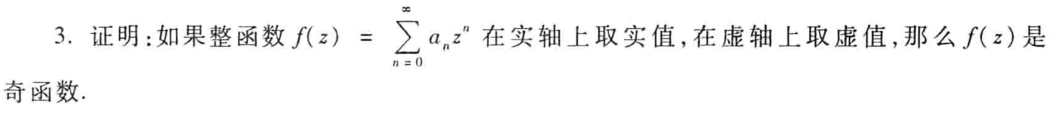
\includegraphics[width=\textwidth]{6-hw14-2025052917.png}
% \caption{}
\label{}
\end{figure}
\end{exercise}
\begin{theorem}[唯一性原理]
设 $f$ 和 $g$ 是区域 $D$ 上的解析函数。如果存在 $D$ 中的一个非空开集 $U$,使得对于所有 $z \in U$ 都有 $f(z) = g(z)$,那么对于所有 $z \in D$ 都有 $f(z) = g(z)$。
\end{theorem}
\begin{theorem}[对称原理]
设 $G \subset \mathbb{C}$ 是一个区域, 并且 $G \cap \mathbb{R} \neq \varnothing$. 记 $G^{+}=\{z \in G: \operatorname{Im} z>0\}$, 且假设 $f: G^{+} \rightarrow \mathbb{C}$ 是解析的, 并且对于每个 $x \in G \cap \mathbb{R}$, 极限 $\lim _{z \rightarrow x} f(z)$ 存在, 且为实数. 那么存在一个解析函数 $\tilde{f}: G \cup G^{*} \cup(G \cap \mathbb{R}) \rightarrow \mathbb{C}$, 使得 $\tilde{f}(z)=f(z)$, 对所有 $z \in G^{+}$成立. 这里 $G^{*}=\{z: \overline{z} \in G\}$, 且对 $z \in G^{-}$有 $\tilde{f}(z)=\overline{f(\overline{z})}$.
\end{theorem}
由唯一性原理,我们可以把下半平面上的 $f(z)$ 看作上半平面的 $f(z)$ 由对称原理解析延拓而来,于是在下半平面上应该有 $f(z)=\overline{f(\overline{z})}$.
\[
\sum_{n=0}^{\infty} a_nz^{n}=\overline{\sum_{n=0}^{\infty} a_n\overline{z}^{n}}=\sum_{n=0}^{\infty} \overline{a_n}z^{n}
\]
于是 $a_n$ 都是实数. 由于 $f(z)$ 在虚轴上取虚值,对于任意实数 $x$,我们有
\[
f(xi)=-\overline{f(x i)}
\]
也就是
\[
\sum_{n=0}^{\infty} a_n(xi)^{n}=-\sum_{n=0}^{\infty} a_n(-xi)^{n}
\]
由 $x$ 的任意性可知, $a_n=(-1)^{n-1}a_n$,于是对于偶数 $n$,我们有 $a_n=0$. 从而
\[
f(z)=\sum_{n=0}^{\infty} a_{2n+1}z^{2n+1}
\]
从而 $f(z)=f(-z)$,$f$ 是奇函数.
